\documentclass[12pt,tikz]{standalone}

\usepackage{graphicx}
\usetikzlibrary{positioning}
\begin{document}

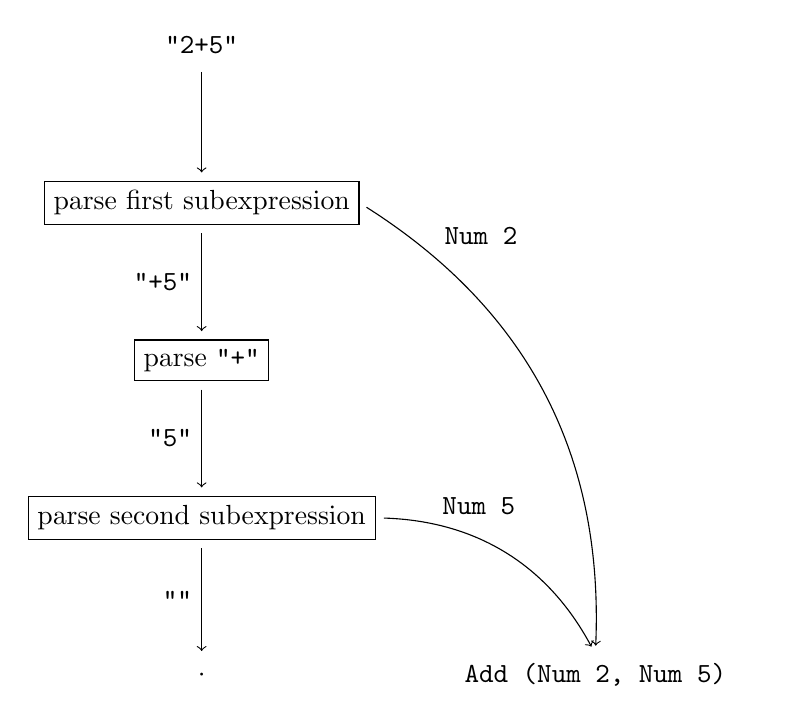
\begin{tikzpicture}[draw, ->, black, node distance = 2cm, shorten >=3pt, shorten <=3pt]
  \newcommand{\xstart}{3}
  \node at (10, 0) (dummy) {};
  \node at (\xstart, 0) (input) {\texttt{"2+5"}};

  \node[draw, black, rectangle] at (\xstart, -2) (subexp1) {parse first subexpression};

  \node[draw, black, rectangle] at (\xstart, -4) (plus) {parse \texttt{"+"}};

  \node[draw, black, rectangle] at (\xstart, -6) (subexp2) {parse second subexpression};

  \node at (\xstart, -8) (finish) {$\cdot$};
  \node at (8, -8) (finalexp) {\texttt{Add (Num 2, Num 5)}};

  \draw (input) -- (subexp1);
  \draw (subexp1) -- node[left] {\texttt{"+5"}} (plus);
  \draw (plus) -- node[left] {\texttt{"5"}} (subexp2);
  \draw (subexp2) -- node[left] {\texttt{""}} (finish);

  \draw (subexp1.east) to[bend left=30] node[right=10pt, pos=0.1] {\texttt{Num 2}} (finalexp.north);
  \draw (subexp2.east) to[bend left=30] node[right=10pt, yshift=5pt, pos=0.1] {\texttt{Num 5}} (finalexp.north);

\end{tikzpicture}

\end{document}
